\section{DETESTS-Dis}

\begin{frame}{Task descriptions}
    \only<1>{
    \begin{columns}
    \column{0.5\textwidth}
    \centering
    \begin{itemize}
        \item Second edition of DETESTS
        \item Stereotype detection on text
        \item Framed within LeWiDi: 
        \begin{itemize}
            \item Aggregated annotations: majority voting and softmax
            \item Non-aggregated annotations
        \end{itemize}
        \item Two tasks:
            \begin{itemize}
                \item \textbf{Stereotype detection}: binary classification task 
                \item \textbf{Stereotype implicitness detection}: novel hierarchy classification task 
            \end{itemize}
        \footfullcite{detests_dis_2024}
    \end{itemize}

    \column{0.5\textwidth}
    \centering
    \includesvg[width=0.8\textwidth]{images/DETEST-tareas.svg}
        \begin{table}[]
            \small
            \centering
            \resizebox{\textwidth}{!}{%
            \begin{tabular}{|c|c|c|}
            \hline
            Task       & Hard evaluation & Soft evaluation \\ \hline
            Stereotype & F1              & CE              \\ \hline
            Implicit   & ICM             & ICM Soft        \\ \hline
            \end{tabular}
            }
        \end{table}
    \end{columns}
    }
    \only<2>{
        \begin{table}[]
            \centering
            \begin{tabularx}{\textwidth}{|X|c|c|}
            \hline
            \textbf{Text} & \textbf{Stereotype} & \textbf{Implicitness} \\ \hline
            The solution is to develop a critical and esceptical thinking. & X & - \\ \hline
            Like it or not, one thing is clear: if there were no muslims in Europe, this wouldn't happen. & \checkmark & X \\ \hline
            Yesterday I was at the tax office, all Spaniards, in the afternoon I went to the health center, half of them Spaniards. & \checkmark & \checkmark \\ \hline
            \end{tabularx}
        \end{table}
    }
\end{frame}

\begin{frame}{Dataset}
   \only<1>{
    \begin{itemize}
        \item Comment threads from news articles
        \item Annotated by 3 expert annotators (2 linguistics and 1 researcher)
        \item Two corpora
        \item DETEST corpora:
        \begin{itemize}
            \item Corpus from the first edition
            \item Threads from online news forums
            \item Annotations are provided on a sentence level
        \end{itemize} 
        \item StereoHOAX corpora:
        \begin{itemize}
            \item New corpora for this edition
            \item Threads from Twitter
            \item Annotations are provided on a tweet level
        \end{itemize}
        \item Different levels of context:
        \begin{itemize}
            \item \textbf{Level 1}: Previous sentence (DETEST)
            \item \textbf{Level 2}: Previous tweet/comment
            \item \textbf{Level 3}: First tweet/comment
            \item \textbf{Level 4}: News text
        \end{itemize}
    \end{itemize}
   }
   
    \only<2>{
        \begin{columns}[T]
        \column{0.5\textwidth}
        \centering
        Stereotype identification
        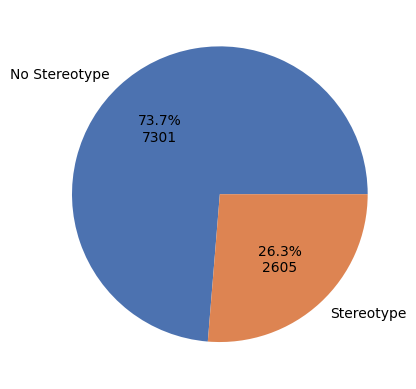
\includegraphics[width=\textwidth]{images/detest_hard_labels.png}

        \column{0.5\textwidth}
        Implicitness detection
        \centering
        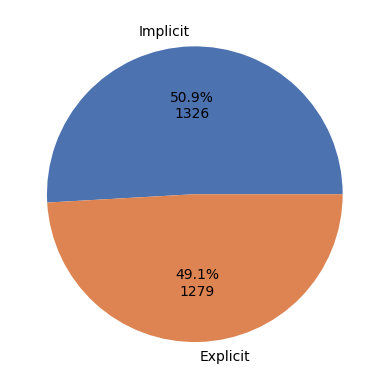
\includegraphics[width=\textwidth]{images/detest_soft_labels.png}
        \end{columns}
    }

\end{frame}

\begin{frame}{System proposals}
    \only<1> {
    \begin{columns}
    \column{0.6\textwidth}
    \begin{itemize}
        \item RoBERTa model as text encoder.
        \item \textbf{Hard label} approach
        \begin{itemize}
            \item Classic approach (comparison purposes)
            \item $\mathcal{L}(\hat{y}, y) = \text{BCE}(\hat{y}, y)$
        \end{itemize}
        \item \textbf{Soft label} approach
        \begin{itemize}
            \item Train by soft label probablity distribution
            \item $\mathcal{L}(\hat{y}, y) = \text{CE}(\hat{y}, y)$
        \end{itemize}
        \item \textbf{Perspectivist} approach
        \begin{itemize}
            \item \textbf{Multi-task proposal}: three classification heads with one output neuron each
            \item $\mathcal{L}(\hat{y}, y) = \sum_{a=1}^{3} \text{CE}(\hat{y_a}, y_a)$
            \item Aggregate outputs for predictions (majority voting and softmax)
        \end{itemize}
    \end{itemize}
    
    \column{0.4\textwidth}
    \centering
    \includesvg[width=4.5cm]{images/DETESTS-dis_presentacion.svg}
    \end{columns}
    }

    \only<2> {
    \begin{columns}
    \column{0.6\textwidth}
    \begin{itemize}
        \item Layer-Wise Learning Rate fine-tuning
        \begin{itemize}
            \item Deeper encoder layers recieve larger updates, shallowers receive smaller ones
            \item $\eta = \{1e-5, 2e-5, 5e-5, 1e-4\}$
            \item $\xi = \{1'0, 0'97, 0'95, 0'90\}$
        \end{itemize}
        \item Context inclusion:
        \begin{itemize}
            \item Append context via [SEP] token
            \item \textbf{DETEST} samples $\rightarrow$ Previous sentence
            \item \textbf{StereoHOAX} samples $\rightarrow$ First tweet
        \end{itemize}
        \item Back-translation on minority class (ES $\rightarrow$ EN $\rightarrow$ ES)
    \end{itemize}

    \column{0.4\textwidth}
    \centering
    \includesvg[width=4.5cm]{images/DETESTS-dis_presentacion.svg}
    \end{columns}
    }
\end{frame}


\begin{frame}{Stereotype detection: train}
    \only<1>{
    \begin{table}[H]
        \centering
        \resizebox{\textwidth}{!}{
        \begin{tabular}{c|cc|c|c}
                     & \multicolumn{2}{c|}{Hiperparámetros} & Hard Evaluation     & Soft evaluation     \\ \hline
        Architecture & \multicolumn{1}{c|}{$\xi$}  & $\eta$ & F1-Stereotype  $\uparrow$     & \textit{Cross Entropy} $\downarrow$                 \\ \hline
        \textit{Hard label}   & \multicolumn{1}{c|}{1.0}    & 1e-5   & 0.7380 $\pm$ 0.0222 & \textbf{0.6260 $\pm$ 0.0157} \\ \hline
        \textit{Hard label}   & \multicolumn{1}{c|}{0.95}   & 1e-5   & \textbf{0.7410 $\pm$ 0.0184} & 0.6308 $\pm$ 0.0125 \\ \hline \hline
        \textit{Soft label}   & \multicolumn{1}{c|}{1.0}    & 5e-5   & 0.7413 $\pm$ 0.0203 & 0.5979 $\pm$ 0.0250 \\ \hline
        \textit{Soft label}   & \multicolumn{1}{c|}{0.95}   & 5e-5   & \textbf{0.7488 $\pm$ 0.0175} & \textbf{0.5926 $\pm$ 0.0169} $\dagger$ \\ \hline \hline
        \textit{Multi-Task}   & \multicolumn{1}{c|}{1.0}    & 2e-5   & 0.7342 $\pm$ 0.0308 & 0.8191 $\pm$ 0.0411 \\ \hline
        \textit{Multi-Task}   & \multicolumn{1}{c|}{0.90}   & 2e-5   & \textbf{0.7519 $\pm$ 0.0163} $\dagger$ & \textbf{0.8094 $\pm$ 0.0350} \\ \hline
        \end{tabular}%
        }
        \caption{Comparison of normal fine-tuning with the best parameters found on hyperparameter search.}
        %\label{tab:detests_dis_hiper}
        \end{table}
    }
    \only<2>{
        \begin{columns}
            \column{0.55\textwidth}
            \centering
            Hard label approach
            \adjustbox{max width=\textwidth}{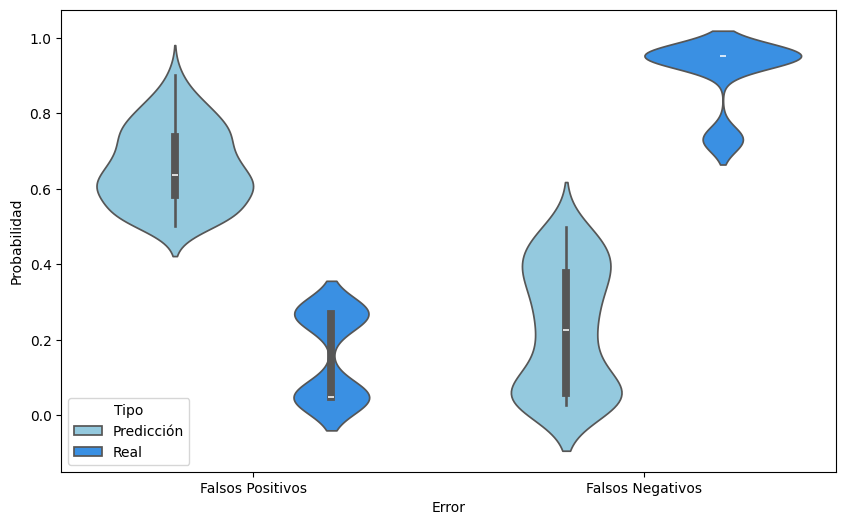
\includegraphics{images/violin_plot_hard.png}}
            
            \column{0.55\textwidth}
            \centering
            Soft label approach
            \adjustbox{max width=\textwidth}{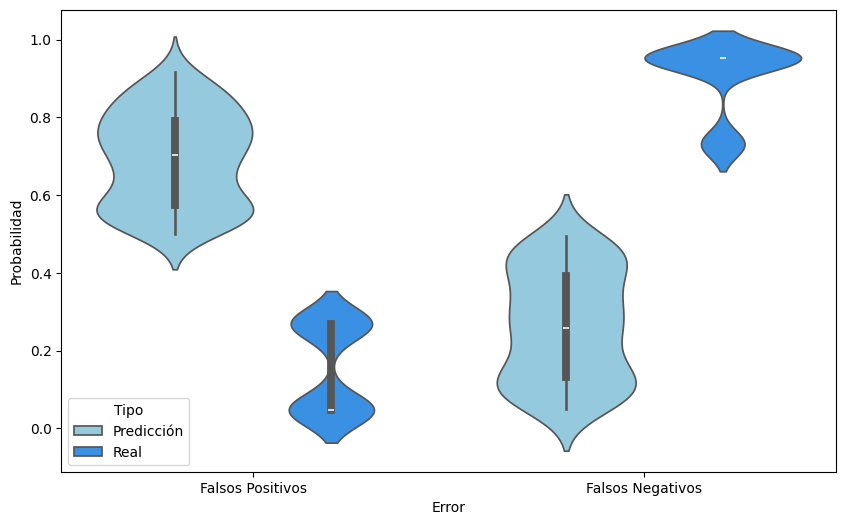
\includegraphics{images/violin_plot_soft.png}}
            
        \end{columns}
    }

    \only<3>{
        \centering
        Perspectivist approach
        \adjustbox{max width=\textwidth}{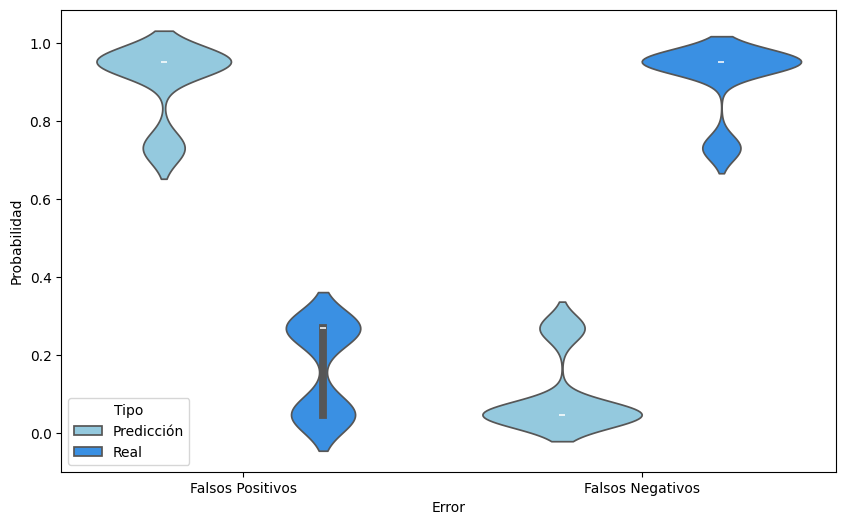
\includegraphics{images/violin_plot_annotators.png}}
    }
    \only<4>{
        \begin{table}[H]
            \centering
            \resizebox{\textwidth}{!}{
            \begin{tabular}{c|c|c}
                         & Hard Evaluation          & Soft evaluation     \\ \hline
            Architecture & F1-Stereotype $\uparrow$ & \textit{Cross Entropy} $\downarrow$     \\ \hline
            \textit{Hard label}   & 0.8713 $\pm$ 0.0081      & 0.6588 $\pm$ 0.0397 \\ \hline
            \textit{Soft label}   & 0.8980 $\pm$ 0.0046  $\dagger$    & 0.5177 $\pm$ 0.0076 $\dagger$ \\ \hline
            \textit{Multi-Task}   & 0.8829 $\pm$ 0.0084      & 0.6369 $\pm$ 0.0289 \\ \hline
            \end{tabular}
            }
            \caption{Back translation alongside context with each archicecture. $\dagger$ highlights the best results for each evaluation.}
            \label{tab:detests_dis_data_context_and_aug}
            \end{table}
    }

\end{frame}
\begin{frame}{Stereotype detection results: test}
    \begin{table}[hbt]
    \centering
    \resizebox{\textwidth}{!}{%
    \begin{tabular}{c|cc||cc|}
    \cline{2-5}
                                              & \multicolumn{2}{c||}{Hard evaluation}                       & \multicolumn{2}{c|}{Soft evaluation}                                      \\ \hline
    \multicolumn{1}{|c|}{Architecture}        & \multicolumn{1}{c|}{\# ranking/21} & F1 Score $\uparrow$ & \multicolumn{1}{c|}{\# ranking/8} & \textit{Cross Entropy} $\downarrow$ \\ \hline
    \multicolumn{1}{|c|}{\textit{Hard label}} & \multicolumn{1}{c|}{7}               & 0.653               & \multicolumn{1}{c|}{8}              & 1.409                               \\ \hline
    \multicolumn{1}{|c|}{\textit{Soft label}} & \multicolumn{1}{c|}{\textbf{4}}      & \textbf{0.691}      & \multicolumn{1}{c|}{\textbf{2}}     & \textbf{0.850}                      \\ \hline
    \multicolumn{1}{|c|}{\textit{Multi-task}} & \multicolumn{1}{c|}{5}               & 0.685               & \multicolumn{1}{c|}{7}              & 1.081                               \\ \hline \hline
    \multicolumn{1}{|c|}{Gold baseline}       & \multicolumn{1}{c|}{0}               & 1.000               & \multicolumn{1}{c|}{0}              & 0.255                               \\ \hline
    \multicolumn{1}{|c|}{Winners}           & \multicolumn{1}{c|}{1}               & 0.720               & \multicolumn{1}{c|}{1}              & 0.841                               \\ \hline
    \multicolumn{1}{|c|}{Baseline BETO}       & \multicolumn{1}{c|}{6}               & 0.663               & \multicolumn{1}{c|}{4}              & 0.893                               \\ \hline
    \end{tabular}%
    }
    \caption{DETEST-Dis stereotype detection official test results. Our best results are highlighted in bold for each evaluation.}
    \label{tab:t1_detests}
    \end{table}
    \footfullcite{detests_dis_2024}
\end{frame}



\begin{frame}{Implicitness detection results: train}
    \only<1>{
        \begin{table}[hbt]
            \centering
            \resizebox{\textwidth}{!}{
            \begin{tabular}{c|cc|cc}
                                              & \multicolumn{2}{c|}{Hard evaluation}                        & \multicolumn{2}{c}{Soft evaluation}                                 \\ \hline
            \multicolumn{1}{c|}{Arquitectura} & \multicolumn{1}{c|}{ICM $\uparrow$}   & ICM Norm $\uparrow$ & \multicolumn{1}{c|}{ICM Soft $\uparrow$} & ICM Soft Norm $\uparrow$ \\ \hline
            \multicolumn{1}{c|}{\textit{Hard label}}   & \multicolumn{1}{c|}{\textbf{0.0095 $\pm$ 0.0726}}  & \textbf{0.5049 $\pm$ 0.0533}     & \multicolumn{1}{c|}{0.4277 $\pm$ 0.1586}     & 0.5632 $\pm$ 0.0238          \\ \hline
            \multicolumn{1}{c|}{\textit{Soft label}}   & \multicolumn{1}{c|}{-0.0459 $\pm$ 0.0748} & 0.4644 $\pm$ 0.0568     & \multicolumn{1}{c|}{0.0870 $\pm$ 0.3862}     & 0.5129 $\pm$ 0.0568          \\ \hline
            \multicolumn{1}{c|}{\textit{Multi-task}}   & \multicolumn{1}{c|}{-0.0498 $\pm$ 0.1230} & 0.4649 $\pm$ 0.0891     & \multicolumn{1}{c|}{\textbf{0.4981 $\pm$ 0.3719}}     & \textbf{0.5726 $\pm$ 0.0543}         
            \end{tabular}%
            }
            \caption{Train results for the implicitness detection task of DETEST-Dis. Our best results are highlighted in bold for each evaluation.}
            \end{table}
    }
    \only<2>{
        \begin{table}[hbt]
            \centering
            \begin{tabular}{c|c}
            Architecture & \textit{Cross Entropy} $\downarrow$          \\ \hline
            \textit{Hard label}  & 0.6639 ± 0.0208          \\ \hline
            \textit{Soft label}   & \textbf{0.6282 ± 0.0147} \\ \hline
            \textit{Multi-task}   & 0.8567 ± 0.0902         
            \end{tabular}%
            \caption{Cross-entropy training results for the DETEST-Dis implicitness detection task. Our best results are highlighted in bold.}
            \label{tab:results_detests_ce_t2}
        \end{table}
    }
\end{frame}


\begin{frame}{Implicitness detection results: test}
\begin{table}[]
    \centering
    \resizebox{\textwidth}{!}{%
    \begin{tabular}{c|ccc||ccc|}
    \cline{2-7}
                                              & \multicolumn{3}{c||}{Hard evaluation}                                                             & \multicolumn{3}{c|}{Soft evaluation}                                                                      \\ \hline
    \multicolumn{1}{|c|}{Architecture}        & \multicolumn{1}{c|}{\# ranking/14} & \multicolumn{1}{c|}{ICM $\uparrow$} & ICM Norm $\uparrow$ & \multicolumn{1}{c|}{\# ranking/6} & \multicolumn{1}{c|}{ICM Soft $\uparrow$} & ICM Soft Norm $\uparrow$ \\ \hline
    \multicolumn{1}{|c|}{\textit{Hard label}} & \multicolumn{1}{c|}{4}               & \multicolumn{1}{c|}{0.045}          & 0.516               & \multicolumn{1}{c|}{2}              & \multicolumn{1}{c|}{-0.917}              & 0.401                    \\ \hline
    \multicolumn{1}{|c|}{\textit{Soft label}} & \multicolumn{1}{c|}{\textbf{2}}      & \multicolumn{1}{c|}{\textbf{0.065}} & \textbf{0.524}      & \multicolumn{1}{c|}{3}              & \multicolumn{1}{c|}{-0.969}              & 0.396                    \\ \hline
    \multicolumn{1}{|c|}{\textit{Multi-task}} & \multicolumn{1}{c|}{3}               & \multicolumn{1}{c|}{0.061}          & 0.522               & \multicolumn{1}{c|}{\textbf{1}}     & \multicolumn{1}{c|}{\textbf{-0.900}}     & \textbf{0.403}           \\ \hline \hline
    \multicolumn{1}{|c|}{Gold baseline}       & \multicolumn{1}{c|}{0}               & \multicolumn{1}{c|}{1.380}          & 1.000               & \multicolumn{1}{c|}{0}              & \multicolumn{1}{c|}{4.651}               & 1.000                    \\ \hline
    \multicolumn{1}{|c|}{Baseline BETO}       & \multicolumn{1}{c|}{1}               & \multicolumn{1}{c|}{0.126}          & 0.546               & \multicolumn{1}{c|}{4}              & \multicolumn{1}{c|}{-1.124}              & 0.379                    \\ \hline
    \end{tabular}%
    }
    \caption{Test results for the implicitness detection task of DETEST-Dis. Our best results are highlighted in bold for each evaluation.}
    \label{tab:t2_detests}
    \end{table}
    \footfullcite{detests_dis_2024}
\end{frame}